\documentclass[table]{cubeamer}
\setbeameroption{show notes on second screen=right} % Both

\usepackage{twemojis}
\usepackage{graphicx}

\newcommand*\annotatedFigureBox[3]{\draw[#3,thick,rounded corners] (#1) rectangle (#2);}
\newenvironment {annotatedFigure}[1]{\centering\begin{tikzpicture}
\node[anchor=south west,inner sep=0] (image) at (0,0) { #1};\begin{scope}[x={(image.south east)},y={(image.north west)}]}{\end{scope}\end{tikzpicture}}

\usetikzlibrary{arrows.meta, calc, fit, positioning, bending}
\makeatletter
\tikzset{
    database/.style={
        path picture={
            \draw (0, 1.5*\database@segmentheight) circle [x radius=\database@radius,y radius=\database@aspectratio*\database@radius];
            \draw (-\database@radius, 0.5*\database@segmentheight) arc [start angle=180,end angle=360,x radius=\database@radius, y radius=\database@aspectratio*\database@radius];
            \draw (-\database@radius,-0.5*\database@segmentheight) arc [start angle=180,end angle=360,x radius=\database@radius, y radius=\database@aspectratio*\database@radius];
            \draw (-\database@radius,1.5*\database@segmentheight) -- ++(0,-3*\database@segmentheight) arc [start angle=180,end angle=360,x radius=\database@radius, y radius=\database@aspectratio*\database@radius] -- ++(0,3*\database@segmentheight);
        },
        minimum width=2*\database@radius + \pgflinewidth,
        minimum height=3*\database@segmentheight + 2*\database@aspectratio*\database@radius + \pgflinewidth,
    },
    database segment height/.store in=\database@segmentheight,
    database radius/.store in=\database@radius,
    database aspect ratio/.store in=\database@aspectratio,
    database segment height=0.1cm,
    database radius=0.25cm,
    database aspect ratio=0.35,
}
\makeatother

\title{Functional Programming}
\subtitle{A lightweight introduction}
\author[Fabio Lonegro]{Fabio Lonegro}
\date{July 13, 2022}

% \institute[Deltatre]{Sport Experiences Unit - Deltatre}

\begin{document}

\maketitle

\cutoc

\section{Functions}

\begin{frame}{Functions}
  \note[item]{Welcome to the talk!}
  \note[item]{As you can see, this slidedeck is a work in progress.}
  \begin{itemize}
    \item Functional programming treats computation as the evaluation of \textit{mathematical functions}
    \pause\item It can take parameters and return a value
    \pause\item It can be called from other parts of the code
  \end{itemize}
\end{frame}

% % \begin{frame}{OMB live components flow}
% %   \begin{tikzpicture}[
% %     process/.style={draw,thick,circle,minimum width=2cm,fill=blue!20},
% %     to/.style={->,>=latex',shorten >=1pt,semithick,font=\sffamily\footnotesize},
% %     cell/.style = {rectangle, draw, very thick, outer sep=0pt,
% %             font=\sffamily\scriptsize},
% %               ]
% %     \begin{scope}[local bounding box=processes]
% %       \node[process] (receiver) {Receiver};
% %       \node[process, right=1cm of receiver] (dispatcher) {Dispatcher};
% %       \node[process, right=1.5cm of dispatcher] (sender1) {$\text{Sender}_\text{1}$};
% %       \node[right=.3cm of sender1] (dots) {$\cdots$};
% %       \node[process, right=.3cm of dots] (sendern) {$\text{Sender}_\text{n}$};
% %     \end{scope}
% %     \begin{scope}
% %       \node[above=1cm of processes] (aux) {KAFKA};
% %       \node[cell,fit=(aux.north-|processes.west)
% %         (aux.south-|processes.east),inner sep=0pt](input){};
% %       \coordinate (ISWT) at($(input.south west)$);

% %       \path (ISWT) +(-15:-1) coordinate (RInT);
% %       \node[draw=red, circle, fill=red, minimum size=5, 
% %         label={[label distance=.3cm,rotate=90, font=\tiny, centered]120:ODF}] (RIn) at($(RInT)$) {};
% %     \end{scope}
% %     \path (sender1) +(90:-2) coordinate (S1OutT);
% %     \path (sendern) +(90:-2) coordinate (SnOutT);
% %     \node[circle, fill=black, label={below:HTTP Receiver}] (S1Out) at($(S1OutT)$) {};
% %     \node[circle, fill=black, label={below:HTTP Receiver}] (SnOut) at($(SnOutT)$) {};
    
% %     \path (ISWT) +(0:2.2) coordinate (RT);
% %     \path (ISWT) +(0:5.7) coordinate (S1T);
% %     \path (ISWT) +(0:9.3) coordinate (SnT);
% %     \draw[to, dashed] (RIn) to (receiver);
% %     \draw[to] (receiver) to[out=-0,in=-90] (RT);
% %     \draw[to] (RT) +(0:.4) to[out=-90,in=-180] (dispatcher);
% %     \draw[to] (dispatcher) to[out=-0,in=-90] (S1T);
% %     \draw[to] (dispatcher) to[out=45,in=-90] (SnT);
% %     \draw[to] (S1T) +(0:.4) to[out=-90,in=-180] (sender1);    
% %     \draw[to] (SnT) +(0:.4) to[out=-90,in=-180] (sendern);
% %     \draw[to, dashed] (sender1) to (S1Out);
% %     \draw[to, dashed] (sendern) to (SnOut);
% %   \end{tikzpicture}
% % \end{frame}

% % Receiver
% \begin{frame}{Receiver key features}
%   \begin{itemize}
%     \item Receives XML feeds through HTTP POST from Omega
%     \pause\item Serializes and puts the content into a Kafka topic
%   \end{itemize}
% \end{frame}
% \begin{frame}{Receiver open points}
%   \begin{itemize}
%     \item Should skip not valid XML?
%   \end{itemize}
% \end{frame}

% % Dispatcher
% \begin{frame}{Dispatcher key features}
%   \begin{itemize}
%     \item Enriches the value of the item in kafka with metadata useful for filtering taken from the header of the feed
%     \pause\item Dispatches each feed to clients based on configuration of the filters
%   \end{itemize}
% \end{frame}
% \begin{frame}{Dispatcher open points}
%   \begin{itemize}
%     \item What filters do we want to make available for the clients?\\i.e. Type,RSC (or part of it),Date...
%   \end{itemize}
% \end{frame}

% % Sender
% \begin{frame}{Sender key features}
%   \begin{itemize}
%     \item Sends each feed to the endpoint configured for the client
%     \pause\item Has an active monitoring for the state of each process
%   \end{itemize}
% \end{frame}
% \begin{frame}{Sender open points}
%   \begin{itemize}
%     \item Should we provide a retry logic?
%     \pause\item Should we provide a throttling logic?
%     \pause\item Should we provide self stats and error checking (i.e. lag,last HTTP error)?
%     \pause\item Should we provide a way for the client to start/stop the live sending?
%   \end{itemize}
% \end{frame}

% \section{OMB BIF}

% \begin{frame}{OMB BIF components flow}
%   \begin{tikzpicture}[
%     process/.style={draw,thick,circle,minimum width=2cm,fill=blue!20},
%     webprocess/.style={draw,thick,circle,minimum width=2cm,fill=green!20},
%     to/.style={->,>=latex',shorten >=1pt,semithick,font=\sffamily\footnotesize},
%     cell/.style = {rectangle, draw, very thick, outer sep=0pt, font=\sffamily\scriptsize}]
%     \def\processdistance{.5cm}
%     \def\symboldistance{.4cm}
%     \def\dotsdistance{.1cm}
%     \setlength{\twemojiDefaultHeight}{20pt}
%     \begin{scope}[local bounding box=bifprocesses]
%       \node[process] (bifindexer) {Bif Indexer};
%       \node[database, database radius=.8cm,database segment height=0.3cm, below right={\processdistance} of bifindexer, 
%         label=below:Relational DB] (database) {};
%       \node[webprocess, above right={\processdistance} of database] (bifweb) {Bif Web};
%       \node[below={\symboldistance} of bifweb] (zip) {$\twemoji{open file folder}$};
%       \node[below right={\symboldistance} of bifweb] (person) {$\twemoji{person}$};
%       \node[process, right={\processdistance} of bifweb] (bifsender1) {$\text{Bif Sender}_\text{1}$};
%       \node[right={\dotsdistance} of bifsender1] (bifdots) {$\cdots$};
%       \node[process, right={\dotsdistance} of bifdots] (bifsendern) {$\text{Bif Sender}_\text{n}$};
%     \end{scope}
%     \begin{scope}
%       \node[above=1cm of bifprocesses] (bifaux) {KAFKA};
%       \node[cell,fit=(bifaux.north-|bifprocesses.west)
%         (bifaux.south-|bifprocesses.east),inner sep=0pt](bifinput){};
%       \coordinate (BISWT) at($(bifinput.south west)$);

%       \path (BISWT) +(-15:-1) coordinate (DInT);
%       \node[draw=blue, circle, fill=blue, minimum size=5, 
%         label={[label distance=.3cm,rotate=90, font=\tiny, centered]120:Dispatcher output}] (DIn) at($(DInT)$) {};

%       \path (BISWT) +(0:1) coordinate (BI);
%       \path (BISWT) +(0:8.2) coordinate (BS1T);
%       \path (BISWT) +(0:11.2) coordinate (BSnT);

%       \path (bifsender1) +(90:-2) coordinate (BifS1OutT);
%       \path (bifsendern) +(90:-2) coordinate (BifSnOutT);
%       \node[circle, fill=black, label={below:HTTP receiver}] (BifS1Out) at($(BifS1OutT)$) {};
%       \node[circle, fill=black, label={below:HTTP receiver}] (BifSnOut) at($(BifSnOutT)$) {};

%       \draw[to, dashed] (DIn) to (bifinput);
%       \draw[to] (BI) to (bifindexer);
%       \draw[to] (bifindexer) to (database);
%       \draw[to] (bifweb) to (database);
%       \draw[to, dotted] (person) to (bifweb);
%       \draw[to, dashed] (bifweb) to (zip);
%       \draw[to] (bifweb) to (BS1T);
%       \draw[to] (BS1T) to (bifsender1);
%       \draw[to] (bifweb) to[out=50,in=-120] (BSnT);
%       \draw[to] (BSnT) to (bifsendern);
%       \draw[to, dashed] (bifsender1) to (BifS1Out);
%       \draw[to, dashed] (bifsendern) to (BifSnOut);
%     \end{scope}
%   \end{tikzpicture}
% \end{frame}

% % BIF Indexer
% \begin{frame}{BIF Indexer key features}
%   \begin{itemize}
%     \item Persists feeds and their associations with clients into the relational database
%   \end{itemize}
% \end{frame}
% \begin{frame}{BIF Indexer open points}
%   \begin{itemize}
%     \item Should we produce periodically archives for each client?\\(i.e. by day, by week, ...)
%     \pause\item Do filters apply backwards in case of change?
%   \end{itemize}
% \end{frame}

% % BIF Web App
% \begin{frame}{BIF Web App key features}
%   \begin{itemize}
%     \item Shows the list of feeds dispatched to the client with filtering options
%     \pause\item Allows the client to request the creation of an archive with selected feeds and download it 
%   \end{itemize}
% \end{frame}
% \begin{frame}{BIF Web App open points}
%   \begin{itemize}
%     \item Should we show here or in another tool "self-care" options for the client?\\(i.e. send stats, errors, start/stop live send, change of the filters...)
%   \end{itemize}
% \end{frame}

% \begin{frame}{BIF feed list example}
%   \begin{tiny}  
%     \textit{The list contains only the feeds dispatched to the client}\\
%   \end{tiny}  
%   \begin{figure}[h!t]
%     \begin{annotatedFigure}
%       {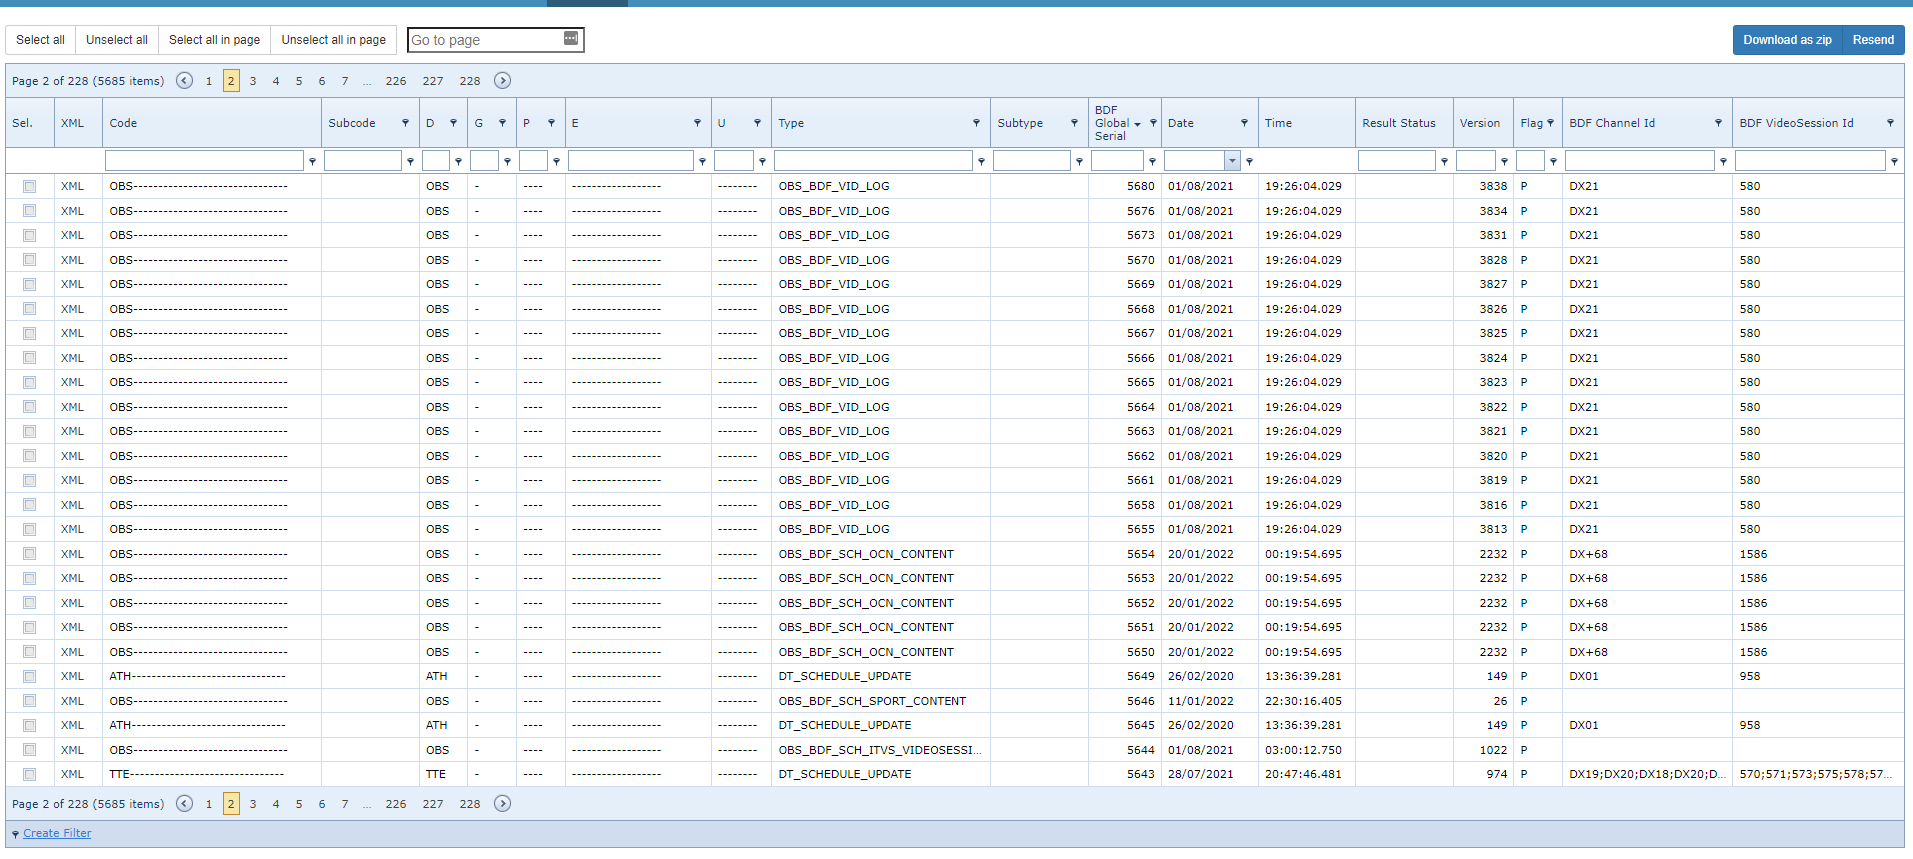
\includegraphics[width = 1\textwidth]{img/bdf-bif-screenshot.png}}
%       \annotatedFigureBox{0.9,0.9242}{0.9988,0.9835}{draw=red}%bl
%       \annotatedFigureBox{-0.0,0.7885}{1,0.8349}{draw=green}
%     \end{annotatedFigure}
%   \end{figure}
% \end{frame}

% \begin{frame}[standout]
% \end{frame}

\end{document}